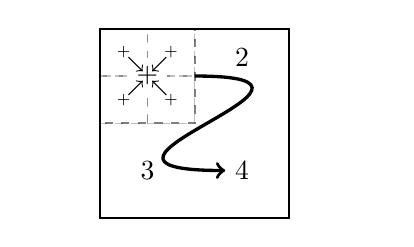
\begin{tikzpicture}[
	scale=0.6,
	adder/.style={
		fill=white
	}
]
	% Initial
	\draw[thick] (0, 0) rectangle ++(4, 4);
	\foreach \x in {0,...,1} {
		\foreach \y in {2,...,3} {
			\draw[dashed, opacity=0.25] (\x, \y) rectangle ++(1, 1);
			\node[adder] at ({\x+0.5}, {\y+0.5}) {\tiny+};
		}
	}
	\draw[dashed, thick, opacity=0.5] (0, 2) rectangle ++(2, 2);
	\node[adder] (tmp) at (1, 3) {+};
	\draw[<-] (tmp.center) ++( 0.1,  0.1) -- ++( 0.3,  0.3);
	\draw[<-] (tmp.center) ++( 0.1, -0.1) -- ++( 0.3, -0.3);
	\draw[<-] (tmp.center) ++(-0.1,  0.1) -- ++(-0.3,  0.3);
	\draw[<-] (tmp.center) ++(-0.1, -0.1) -- ++(-0.3, -0.3);
	\node[anchor=south] (n2) at (3, 3) {2};
	\node (n3) at (1, 1) {3};
	\node (n4) at (3, 1) {4};
	\draw[->, very thick]
		(2, 3) .. controls(6, 3) and (-1.5, 1) .. (n4);
\end{tikzpicture}
